\documentclass[12pt]{article}
\usepackage[spanish]{babel}
% \usepackage{natbib}
\usepackage{url}
\usepackage[utf8]{inputenc}

\usepackage{xfrac}
\usepackage{amsmath}
% \numberwithin{equation}{section}
\usepackage{mathtools}

\usepackage{empheq}
\usepackage{graphicx}
\usepackage{parskip}
\usepackage{fancyhdr}
\usepackage{vmargin}
\usepackage[ddmmyy]{datetime}
\usepackage{anyfontsize}
\usepackage{helvet}
\renewcommand{\familydefault}{phv}
\usepackage{xcolor}

\usepackage{float}
\usepackage[section]{placeins}
\usepackage{tocloft}
\usepackage{listings}

\lstset{
    language=VHDL,
    basicstyle=\ttfamily\small,
    keywordstyle=\color{blue},
    commentstyle=\color{green!60!black},
    stringstyle=\color{red},
    breaklines=true,
    backgroundcolor=\color{gray!05}, % fondo clarito
    frame=none
}


% Alinear completamente el texto del índice de figuras al margen izquierdo
\setlength{\cftfigindent}{0pt}     % sin sangría a la izquierda
\setlength{\cftfignumwidth}{2em}   % ancho reservado para "Figura X"

\setlength{\skip\footins}{5pt}
\usepackage[bottomfloats,belowfloats,hang]{footmisc}

% align first letter of all the lines in the footnotes
\setlength{\footnotemargin}{6pt}

% surround footnotes number with square brackets and always use numbers (even
% inside quoted text)
% https://www.overleaf.com/learn/latex/Footnotes
% \renewcommand*{\thefootnote}{\ [\arabic{footnote}]\ \ }
% \renewcommand*{\thempfootnote}{\ [\arabic{mpfootnote}]\ }

% space between text and footer
\setlength\footskip{40pt}
\setlength{\skip\footins}{20pt}


\usepackage[T1]{fontenc}


\usepackage{arevmath} % no funciona con xelatex/lualatex
\DeclareMathSizes{12}{11}{9}{8}

\usepackage{etoolbox}

\AtBeginEnvironment{align}{
    \vspace{-1.25em}
}

% Definir tamaño por defecto para todas las figuras
\setkeys{Gin}{width=\textwidth, keepaspectratio}

% \setmarginsrb{
%    left margin,
%    top margin,
%    right margin,
%    bottom margin,
%    head height,
%    head sep,
%    foot height,
%    foot skip
% }

\setmarginsrb{3.25 cm}{3.5 cm}{3.25 cm}{3.5 cm}
           {1 cm}{0.75 cm}{1 cm}{1.50 cm}

\definecolor{fiubablue}{HTML}{0085e5}
\usepackage{color}
\usepackage{hyperref}
\hypersetup{
    colorlinks=true, % set true if you want colored links
    linktoc=all,     % set to all if you want sections and subsections linked
    linkcolor=fiubablue, % choose some color if you want links to stand out
    urlcolor=fiubablue,
    citecolor=black
}

\usepackage{subfig}

\usepackage{fancyvrb}
\fvset{xleftmargin=\mathindent}

% code blocks
\usepackage{verbatimbox}
\newenvironment{fullgrayverb}
{\verbbox}
{\endverbbox\par\colorbox{gray!25}{\parbox{\textwidth}{\theverbbox}}\par}

% inline code blocks
\usepackage{tcolorbox}
\newcommand\mystrut{\rule[-3pt]{0pt}{12pt}}
\newtcbox{\code}{on line, boxrule=0pt, boxsep=0pt, top=0pt,
left=0pt, bottom=0pt, right=0pt, colback=gray!25, colframe=white,
fontupper={\ttfamily\mystrut}}

\title{Implementación de Sistema Secuencial en VHDL}          % Titulo del trabajo.
\author{Klöckner, Martin Javier}
\date{\today}                   % Fecha (automática)

\makeatletter
\let\thetitle\@title
\let\theauthor\@author
\let\thedate\@date
\makeatother

\pagestyle{fancy}
\fancyhf{}
\rhead{\theauthor}
\lhead{\thetitle}
\cfoot{\thepage}

\renewcommand{\to}{\mathrel{\scriptstyle\rightarrow}}

\begin{document}
\begin{titlepage}
    \vspace*{-2.5cm}
    {\centering
    
\includegraphics[width=1.00\textwidth]{img/logofiuba.png}\\[2.25 cm]}
    \centering
    \textsc{\Large TA147}\\[0.2 cm]
    \textsc{\large Taller de Sistemas Digitales}\\[4 cm]
    \textcolor{cyan}{{
        \fontsize{25}{32}\selectfont \bfseries \thetitle
    }}\\[0.5cm]
    \vspace{1em}
    {\Large \bfseries Primer Trabajo Práctico}\\[5cm]

    \vfill
    \noindent\makebox[\linewidth]{\rule{\textwidth}{0.4pt}}\\[0.5cm]
    \begin{minipage}{.49\textwidth}
    \textbf{Alumno}\\
    Klöckner, Martin Javier
    \end{minipage}%
    \begin{minipage}{.01\textwidth}
    % \centering\textbf{Legajo}\\
    % 105378 
    \end{minipage}%
    \vspace{1em}
    \begin{minipage}{.50\textwidth}
     \begin{flushright}
        \textbf{Correo electrónico}\\
         \href{mailto:mklockner@fi.uba.ar}{mklockner@fi.uba.ar} \\
      \end{flushright}
    \end{minipage}
\end{titlepage}

\setcounter{tocdepth}{2}
\hypersetup{linkcolor=black} % colorlinks=true option is used
\tableofcontents
\listoffigures
\pagebreak

% En el presente trabajo se realiza la implementación y sintesis de un dispositivo
% secuencial que permite controlar dos semaforos en una interseccion de calles.

En el presente trabajo se realiza el diseño, simulación y síntesis de un
sistema digital destinado al control de dos semaforos en una intersección. Se
emplea el lenguaje de descripción de hardware VHDL para modelar el sistema y la
herramienta de linea de comandos GHDL para la compilación y simulación del
diseño. Por ultimo se utliza Xilinx Vivado para reliazar una sintesis sobre el
dispositivo xc7a15tftg256-1.

\hypertarget{introduccion}{%
\section{Introducción}\label{introduccion}}

% Por definición, la transferencia $H(s)$ de un sistema, es el cociente entre la
% entrada $X(s)$ y la salida $Y(s)$ del sistema, suponiendo que todas las
% condiciones iniciales son nulas, específicamente en el dominio de
% Laplace.\footnotemark[1]
El control de tráfico en intersecciones es un problema clásico en sistemas
digitales. La implementación mediante hardware programable permite obtener
soluciones eficientes, determinísticas y además flexibles.

El objetivo del trabajo, entonces, es diseñar e implementar un sistema digital
que controle el estado de dos semaforos en la intersección de dos calles.

\hypertarget{diseño}{%
\section{Diseño}\label{diseño}}

Para la implementacion del control de los dos semaforos se modela al sistema
como una maquina de estados finita compuesta de seis estados ciclicos, en la que
cada estado representa una configuración de luces. El diagrama de estados de la
maquina de estados diseñada se muestra en la figura \ref{waveform_view}.

\begin{figure}[!ht]
    \centering
    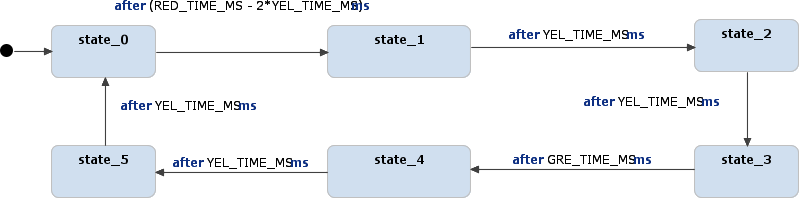
\includegraphics[width=1.00\textwidth]{img/statechart_trim.png}
    \caption{Diagrama de estados del control de semaforos}
    \label{waveform_view}
\end{figure}

Para este trabajo se considera que el estado de cada semaforo es, ordenados en
orden secuencial: solo luz roja encendia, luz roja y amarilla encendida al mismo
tiempo, solo luz verde encendida y solo luz amarilla encendida. Y los estados de
la maquina de estados representas la configuración de luces como se muestra a
continuación

\begin{itemize}
    \item state\_0: primer semaforo en rojo, segundo en verde.
    \item state\_1: primer semaforo en rojo, segundo en amarillo.
    \item state\_2: primer semaforo en rojo y amarillo, sngundo en rojo.
    \item state\_3: primer semaforo en verde, segundo en rojo.
    \item state\_4: primer semaforo en amarillo, segundo en rojo.
    \item state\_5: primer semaforo en rojo, segundo en rojo y amarillo.
\end{itemize}

A cada estado del semanforo se asigna un valor de tiempo en segundos, para los
estados solo rojo o solo verde se asigna 30 segundos y para los estados que
involucran amarillo se asignan 2 segundos.

Dado que el dispositivo programable en el cual se sintetizará el diseño solo
dispone de una señal de reloj de frecuencia 50 MHz, se implementa un modulo de
reloj de tiempo real (Real Time Clock, RTC) que permita determinar cuandos
milisegundos reales pasan en cada estado. Esto se hacen contando los ciclos de
reloj, sabiendo que el contando se incrementa cada $1/50MHz$ segundos.

\if{0}
\section{Diseño en VHDL}

\subsection{Entidad}
\begin{lstlisting}
entity semaforo is
    Port (
        clk     : in  STD_LOGIC;
        reset   : in  STD_LOGIC;
        luz_A   : out STD_LOGIC_VECTOR (2 downto 0);
        luz_B   : out STD_LOGIC_VECTOR (2 downto 0)
    );
end semaforo;
\end{lstlisting}

\subsection{Arquitectura}
\begin{lstlisting}
architecture Behavioral of semaforo is

type estado_type is (S0, S1, S2, S3);
signal estado : estado_type := S0;

begin

process(clk, reset)
begin
    if reset = '1' then
        estado <= S0;
    elsif rising_edge(clk) then
        case estado is
            when S0 => estado <= S1;
            when S1 => estado <= S2;
            when S2 => estado <= S3;
            when S3 => estado <= S0;
        end case;
    end if;
end process;

process(estado)
begin
    case estado is
        when S0 =>
            luz_A <= "100"; -- Verde
            luz_B <= "001"; -- Rojo
        when S1 =>
            luz_A <= "010"; -- Amarillo
            luz_B <= "001";
        when S2 =>
            luz_A <= "001"; -- Rojo
            luz_B <= "100"; -- Verde
        when S3 =>
            luz_A <= "001";
            luz_B <= "010"; -- Amarillo
    end case;
end process;

end Behavioral;
\end{lstlisting}
\fi

\hypertarget{simulacion}{%
\section{Simulación}\label{simulacion}}

Para realizar la simulacion se creó un nuevo módulo en el cual se encapsula el
sistema diseñado, esto de manera de proporcionar señales ficticias que actuen
como entradas y salidas. En particular, para la señal de reloj, se utilizó un
reloj de frecuencia 1 MHz, pero se "engaño" al moudlo rtc para que cuente hasta
$1/1000$ veces la frecuencia de reloj. De esta forma, un segundo de tiempo
"real" se tranforma en un milisegundo de tiempo de simulación.

Como herramientas de simulación se utilizó \emph{GHDL} y \emph{make} para
organizar el proceso de analisis, elaboracion y simulacion del sistema, luego
durante la sintesis, Vivado tambien proporciona una opción de simulación
utilizando los mismos módulos. Para la visualización de las señales se utilizó
\emph{surfer}, el cual es un programa similar a \emph{GTKWave}. El resultado de
la simulacion se muestra en la figura \ref{waveform_view} a continuación.

\begin{figure}[!ht]
    \centering
    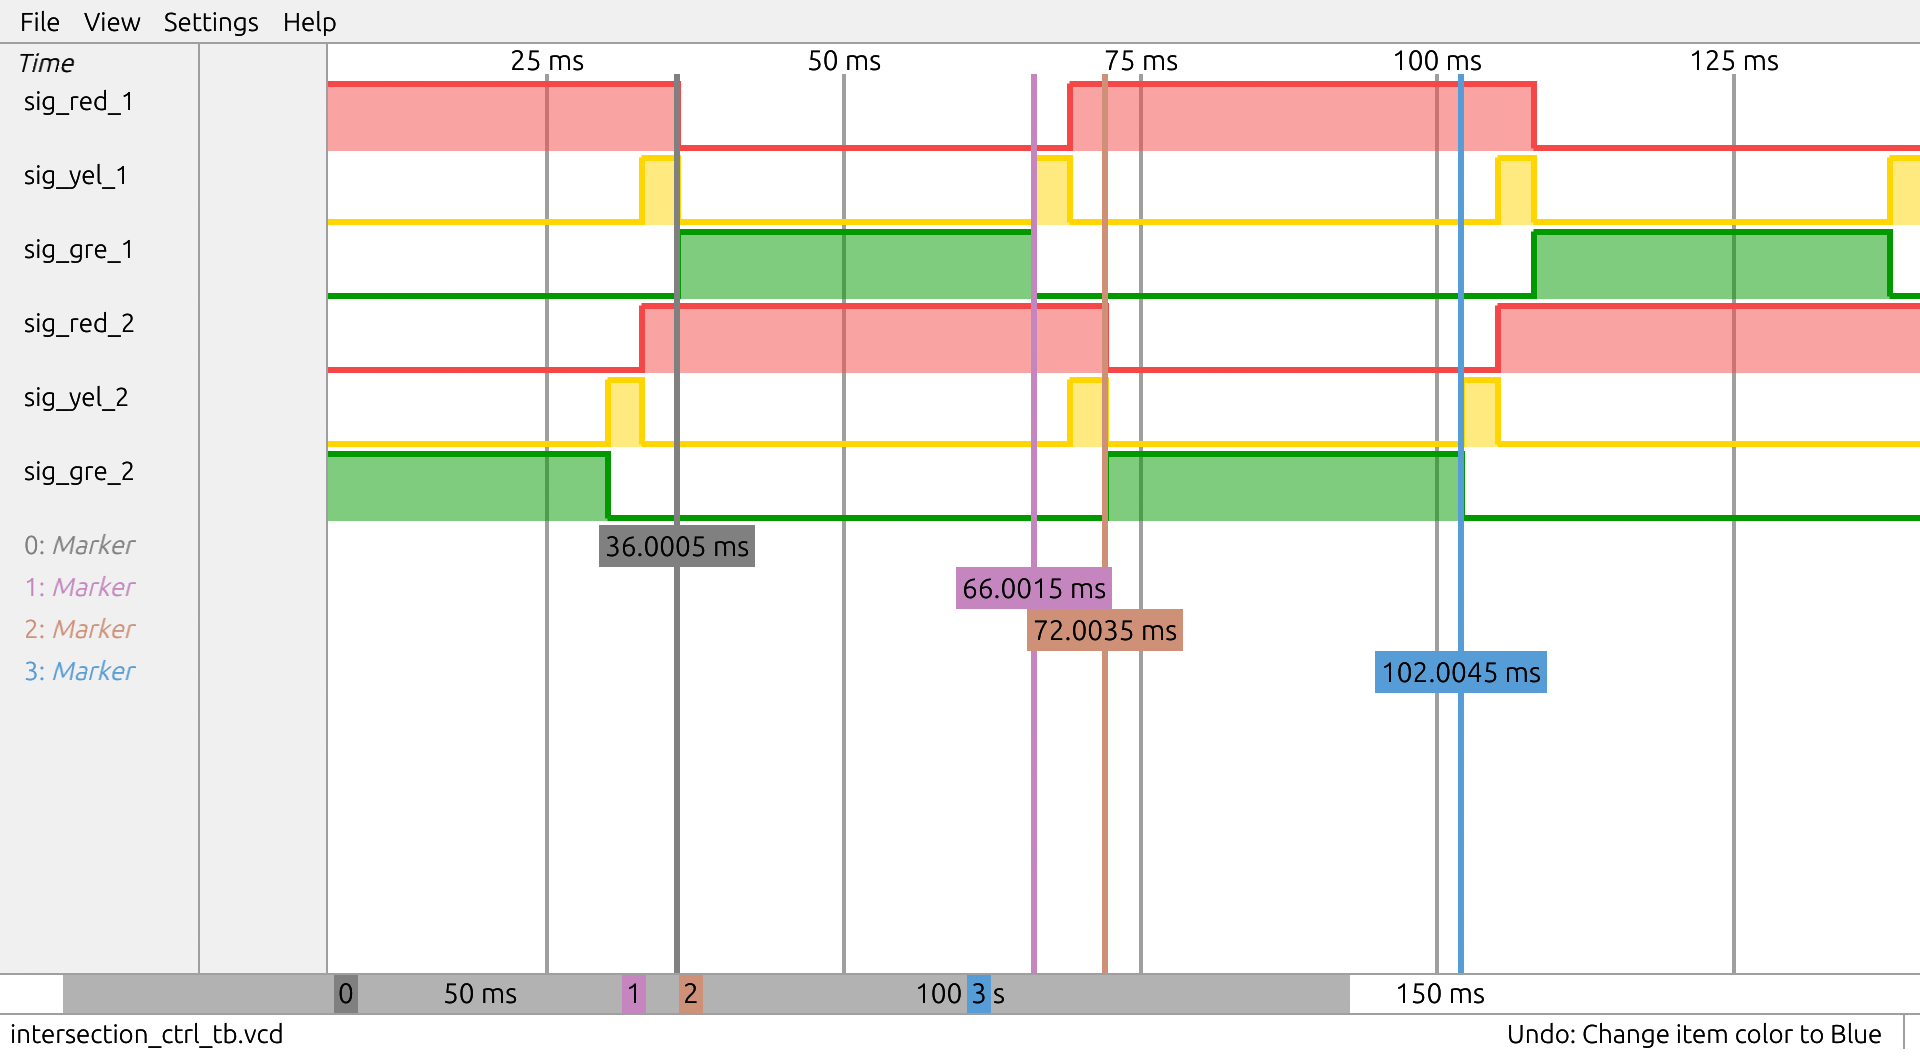
\includegraphics[width=1.00\textwidth]{img/waveform_view_whiter.png}
    \caption{Resultado de las señales simuladas}
    \label{waveform_view}
\end{figure}

\hypertarget{sintesis}{%
\section{Síntesis}\label{sintesis}}

Utilizando Vivado se realizo una sintesis del sistema sobre el dispositivo FPGA
modelo xc7a15tftg256-1.

% \begin{itemize}
%     \item No existen bucles combinacionales.
%     \item El diseño es completamente sincrónico.
%     \item Se utilizan registros adecuados.
% \end{itemize}

\hypertarget{conclusion}{%
\section{Conclusión}\label{conclusion}}

En este trabajo se logró implementar un controlador de dos semaforos parala
intersección de dos calles utilizando VHDL y validando el diseño mediante
simulación en GHDL. Luego se realizo una sintesis utilizando Vivado. Con
respecto a las maquinas de estados finitos, se concluye que resultan adecuadas
para este tipo de aplicaciones.

\end{document}
